% Created 2024-11-24 Sun 22:09
% Intended LaTeX compiler: pdflatex
\documentclass[11pt]{article}
\input{../../../preamble.tex}
% setting up title page
\usepackage{svg}
\title{
  
\includegraphics[width=0.4\textwidth]{fmf_logo}\\
  {\small Oddelek za fiziko} \\
  {Poskusi z žarki X}\\
  {\small Poročilo pri FP5}\\
}
\date{}
\author{ Kristofer Č. Povšič, 28211104 \\[5 cm]
 \small  Asistent: Tilen Knaflič \\
}
\addbibresource{refs.bib}

\begin{document}

\maketitle
\newpage
\tableofcontents
\newpage
\section{Uvod}\label{sec:org9821085}
\subsection{Izvor žarkov X}\label{sec:org77d27ca}
Elektrone iz katode pospešimo z visoko napetostjo proti kovinski tarči. Pri trku zaradi zaviranje elektronov v polju jeder pride do zavornega sevanja v spektru žarkov X.

Elektroni, ki imajo zadosti energije, pa iz notranjih elektronskih lupin gradnikov izbijejo elektrone. Elektroni iz višjih stanj zapolnijo vrzel, pri tem pa izsevajo karakteristične X žarke, ki imajo točno določeno energijo.
\subsection{Ionizacijska celica}\label{sec:org639605f}
Najenostavnejša ionizacijska celica je ploščni kondenzator zvezan z izvorom visoke napetosti. Če v prostor med ploščama posvetimo z rentgenskimi žarki, ti na atomih zraka povzročijo fotoefekt. Fotoelektroni zaradi svoje visoke hitrosti ionizirajo molekule. Nastale ionske pare napetost na kondenzatorju usmeri k ploščam in dobimo tokovni sunek na tokokrogu. Ob zadostni količini fotonov, se sunki povprečijo v merljiv električni tok.

V splošnem ne dosežejo vsi ionski pari elektrod, ker se jih nekaj že prej rekombinira. Pri majhnih jakosti je to znatno, pri višjih pa ne več. To pomeni, da z višanjem narašča tudi tok, nato pa nastopi nasičenje.

Pri rentgenskih napravah pogosto uporabljamo izraz ekspozicijske doze namesto števila fotonov, saj ni pomembno samo število, ampak tudi energija. Ekspozicijska doza \(X\) je električni naboj \(\Delta Q\)enega predznaka, ki ga v zraku volumna \(\Delta V\) z maso \(\Delta m\), na enoto mase sprosti ionizirajoče sevanje

\[ X = \frac{\Delta Q}{\Delta m} 
\]

Enota za ekspozicijsko dozo je \(\frac{\mathrm{As}}{\mathrm{kg}}\). Hitrost doze definiramo z odvodom doze po času in jo izrazimo s tokom:
\begin{equation}\label{eq:1}
\frac{\mathrm{d} X}{\mathrm{d} t} = \frac{\Delta I}{\Delta m} = \frac{\Delta I }{\rho \Delta V}
\end{equation}

\subsection{Polarizacija žarkov X}\label{sec:org794e03d}
Žarki X nastanejo v rentgenski cevi kot posledica interakcije pospešenih elektronov z jedri v anodi.

Frekvenca izsevanega elektromagnetnega valovanja \(\nu\) je določena s kinetično energijo \(\Delta E_k\), ki jo izgubi elektron. Maksimalno frekvenco dobimo, ko se vsa elektronova kinetična energija spremeni v elektromagnetno:

\[  h \nu = E_k
\]
kjer je \(h\) Planckova konstanta. 

Priročna je formula za izračun ustrezne valovne dolžine

\[ \lambda_{min}[nm] = \frac{1240}{U[\mathrm{V}]} 
\]

kjer je \(U\) anodna napetost. Velja, da je pri napetosti \(12.4 \mathrm{kV}\) minimalna valovna dolžina \(0.1 \mathrm{nm}\).

Spekter sevanja žarkov X je po večini zvezen, vendar ima tudi diskretne črte, ki so posledice skakanja višjih elektronov na prazna mesta.

Predpostavimo, da naboj niha v smeri osi \(y\) z nekim pospeškom. Pospeševanju naboja sledi sevanje elektromagnetnega valovanja, ki ga opišemo z vektorjem jakosti električnega polja \(\vec{E}\) (ki ima smer nihajočega naboja in je pravokoten na smer razširjanja valovanja). Ker naboj niha v smeri \(y\), je tja tudi usmerjen \(\vec{E}\). Pravimo, da je valovanje linearno polarizirano.

Energijski tok valovanja, ki ga seva tak nihajoč naboj je največji v ekvatorialni ravnini, v smeri nihanja naboja pa je enak 0.

Če imamo več istočasno nihajočih nabojev, katerih smeri nihanja so enakomerno porazdeljene v ravnini \(yz\), dobimo v smeri \(x\) nepolarizirano valovanje. Če ni enakomerno porazdeljeno, dobimo delno polarizirano svetlobo.

Če bi elektroni v anodi zavirali le v smeri svojega gibanja, bi dobili linearno polarizirane žarke. V resnici se veliko elektronov odkloni od prvotne smeri že prej in zato so žarki le delno polarizirani.

Z merjenjem jakosti elastičenga sipanja valovanja lahko določimo polariziranost rentgenske svetlobe. Gostota energijskega toka, ki ga seva nihajoči naboj se spreminja kot \(\sin ^2 \theta\), kjer je \(\theta\) kot med smerjo nihanja dipola in smerjo valovanja. Pri elastičnem sipanem odbojnem valovanju dobimo močno sevanje v ravnini, ki je pravokotna na smer nihanja naboja, v sami smeri nihanja pa sevanja ni. V snop, ki ima smer osi \(y\) postavimo sipalec, nato pa v ravnini \(xz\) z Geiger-Mullerjevim števcem izmerimo kotno porazdelitev sipanega valovanja. Merimo pravzaprav le dve pravokotni komponenti \(I_x\) in \(I_z\). Polariziranost tako definiramo kot

\begin{equation}\label{eq:2}
 \eta = \frac{I_z - I_x}{I_z + I_x}
\end{equation}


\subsection{Presevno slikanje predmetov}\label{sec:orgbbc0edf}

Žarki X se absorbirajo v snovi, kar opišemo

\[I = I_0 e ^{- \mu d}
\]

kjer je \(\mu\) linearni absorpcijski koeficient in \(d\) dolžina poti žarka X v sredstvu. Ta pojav lahko izkoristimo za rentgensko slikanje.

\section{Potrebščine}\label{sec:org2919fcb}

\begin{itemize}
\item rentgenska naprava
\item ionizacijska celica
\item izvor napetosti
\item upor in voltmeter
\item 2 sipalca
\item GM števec
\item računalnik
\item fotoaparat
\end{itemize}

\section{Naloge}\label{sec:orge92d4a4}
\begin{itemize}
\item Z ionizacijsko celico izmeri povprečno jakost doze v snopu žarkov X (ter hitrost ekspozicijske doze v odvisnosti od anodne napetosti)
\item Izmeri polariziranost primarni žarkov X
\item Izmeri polariziranost sipanih žarkov X
\item Slikaj čim več predmetov v praktikumu
\end{itemize}

\section{Navodila}\label{sec:orgffcac4c}
Po navodilih rentgenske naprave sestavimo ionizacijsko celico.  Za nekaj vrednosti napetosti na rentgenski cevi izmerimo odvisnost toka od napetosti na ionizacijski celici. Zopet po navodili sestavimo postavitvi za enkratno in dvakratno sipanje in izmerimo sunke na GM števcu.


\section{Obdelava podatkov in izračuni}\label{sec:orgdf50172}

Podatke sem shranil v .csv datoteke in jih obdelal s pomočjo Pythona in njegovih knjižnic pandas, uncertainties, numpy in matplotlib.

\subsection{Nasičenost toka v ionizacijski celici ter ekspozicijska doza}\label{sec:org5aad74f}

Meril sem pri treh različnih napetostih v ionizacijski celici in sicer pri \(25 \mathrm{kV}, 30 \mathrm{kV} \text{ in } 35 \mathrm{kV}\). Nasičen tok sem izračunal preko povprečja vrednosti, ki so bile višje od \(U_s = 100 \mathrm{V}\). Prav tako so podatki o nasičenosti toka prikazani v tabeli \ref{tab:ekspo}.

\begin{slika}[H]
\begin{center}
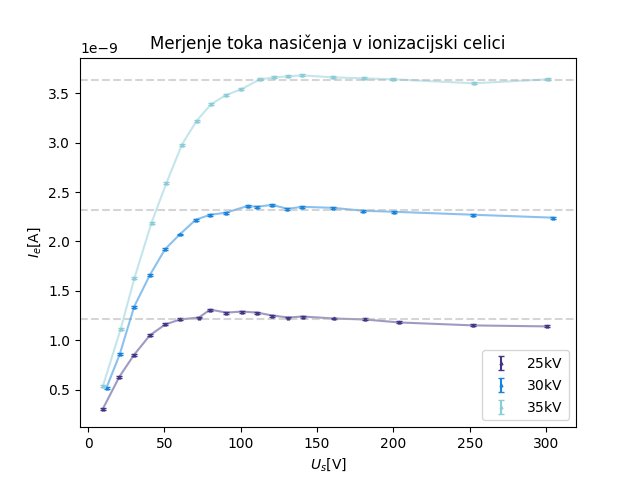
\includegraphics[width=.9\linewidth]{figures/tok_nasicenja.png}
\end{center}
\caption{\small Graf nasičenosti toka pri različnih napetostih v rentgenski cevi.}\label{fig:nasicenost}
\end{slika}
S pomočjo spletnega kalkulatorja \cite{noauthor_air_nodate} sem pri privzetem tlaku \(101 \mathrm{kPa}\) in izmerjeni temperaturi \(22.6 ^{\circ} \mathrm{C}\) ter vlažnosti \(22.7 \%\) izračunal gostota zraka

\[ \rho = 1.18638 \frac{kg}{m ^3}
\]

Ionizacijska celica je v navodilih imela podano vrednost volumna ionizirajočega zraka:

\[ V = 125.4 \mathrm{cm} ^3
\]

Tako sem preko enačbe \ref{eq:1} izračunal sledeče vrednosti za ekspozicijsko dozo povprečenih nasičenih tokov iz tabele \ref{tab:ekspo}
\begin{tabela}[H]
  \centering
\[
  \begin{array}{|c|c|c|}\hline
    U_{R} [\mathrm{kV}] & I_{\text{nasičen}} [\mathrm{nA}] & \dot{X} [\mathrm{mAs/kgh}] \\\hline
    25 & 1.22 \pm 0.05 & (8.1 \pm 0.3) \cdot 10 ^{-6} \\
    30 & 2.32 \pm 0.04 & (1.56 \pm 0.03) \cdot 10 ^{-5} \\
    35 & 3.64 \pm 0.04 & (2.44 \pm 0.03) \cdot 10 ^{-5} \\\hline
    \end{array}
\]
\caption{\small Tabela prikazuje vrednosti nasičenosti toka pri dani napetosti na rentgenski cevi ter pripadajočo izračunano ekspozicijsko dozo.}\label{tab:ekspo}
\end{tabela}

\subsection{Polarizacija primarnih žarkov}\label{sec:orgfe9b6b1}

Postavitev za obe komponenti se vidi na sliki [cite]

\begin{slika}[H]
\begin{center}
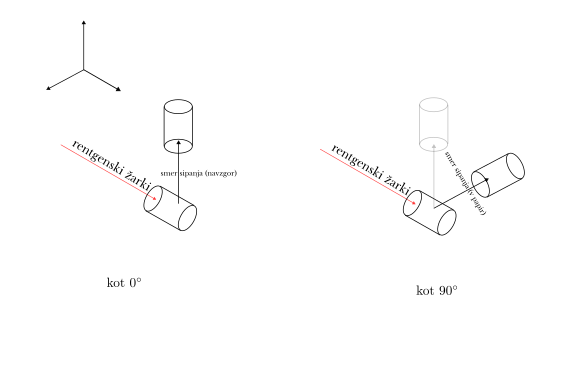
\includegraphics[width=.9\linewidth]{figures/1xsipanje}
\end{center}
\caption{\small Grafika prikazuje postavitev pri enkratnem sipanju, razliko med dvema ravninama. }
\end{slika}

Povprečil sem obe komponenti in dobil
\begin{align*}
  I_x &= 1509.7 \pm 1.9\\
I_z &= 1697.8 \pm 1.7
\end{align*}

Iz tega po definiciji polarizacije \ref{eq:2}

\[ \eta = (0.0586 \pm 0.0008)
\]

Napaka je le grobo ocenjena preko relativne napake obeh komponent.

\subsection{Polarizacija sipanih žarkov}\label{sec:org9f235ad}

Podobno kot za primarne žarke, sem dobil:

\begin{align*}
  I_x &= 2.8 \pm 0.2 \\
I_z &= 0.23 \pm 0.06
\end{align*}

Iz tega po definiciji polarizacije \ref{eq:2} dobim

\[ \eta = 0.8 \pm 0.1
\]

\subsection{Presevno slikanje predmetov}\label{sec:orgf7768b9}

Predmete, ki sem si jih presevno slikal so nalivniki, ključavnica, kvadratasta škatla z neznano vsebino in pa kuli.

\begin{slika}[H]
\begin{center}
\includegraphics[width=.9\linewidth]{figures/kuli.png}
\end{center}
\caption{\small Presevno slikan kemični svinčnik.}
\end{slika}

\begin{slika}[H]
\begin{center}
\includegraphics[width=.9\linewidth]{figures/kroglice.png}
\end{center}
\caption{\small Presevno slikan kvadrat z neznano vsebino.}
\end{slika}

\begin{slika}[H]
\begin{center}
\includegraphics[width=.9\linewidth]{figures/nalivnikInključavnica.png}
\end{center}
\caption{\small Presevno slikana ključavnica in nalivnik.}
\end{slika}

\printbibliography[heading=bibintoc]

\end{document}
